% Options for packages loaded elsewhere
\PassOptionsToPackage{unicode}{hyperref}
\PassOptionsToPackage{hyphens}{url}
\documentclass[
  american,
]{article}
\usepackage{xcolor}
\usepackage[margin=25mm]{geometry}
\usepackage{amsmath,amssymb}
\setcounter{secnumdepth}{5}
\usepackage{iftex}
\ifPDFTeX
  \usepackage[T1]{fontenc}
  \usepackage[utf8]{inputenc}
  \usepackage{textcomp} % provide euro and other symbols
\else % if luatex or xetex
  \usepackage{unicode-math} % this also loads fontspec
  \defaultfontfeatures{Scale=MatchLowercase}
  \defaultfontfeatures[\rmfamily]{Ligatures=TeX,Scale=1}
\fi
\usepackage{lmodern}
\ifPDFTeX\else
  % xetex/luatex font selection
\fi
% Use upquote if available, for straight quotes in verbatim environments
\IfFileExists{upquote.sty}{\usepackage{upquote}}{}
\IfFileExists{microtype.sty}{% use microtype if available
  \usepackage[]{microtype}
  \UseMicrotypeSet[protrusion]{basicmath} % disable protrusion for tt fonts
}{}
\makeatletter
\@ifundefined{KOMAClassName}{% if non-KOMA class
  \IfFileExists{parskip.sty}{%
    \usepackage{parskip}
  }{% else
    \setlength{\parindent}{0pt}
    \setlength{\parskip}{6pt plus 2pt minus 1pt}}
}{% if KOMA class
  \KOMAoptions{parskip=half}}
\makeatother
\usepackage{longtable,booktabs,array}
\usepackage{calc} % for calculating minipage widths
% Correct order of tables after \paragraph or \subparagraph
\usepackage{etoolbox}
\makeatletter
\patchcmd\longtable{\par}{\if@noskipsec\mbox{}\fi\par}{}{}
\makeatother
% Allow footnotes in longtable head/foot
\IfFileExists{footnotehyper.sty}{\usepackage{footnotehyper}}{\usepackage{footnote}}
\makesavenoteenv{longtable}
\usepackage{graphicx}
\makeatletter
\newsavebox\pandoc@box
\newcommand*\pandocbounded[1]{% scales image to fit in text height/width
  \sbox\pandoc@box{#1}%
  \Gscale@div\@tempa{\textheight}{\dimexpr\ht\pandoc@box+\dp\pandoc@box\relax}%
  \Gscale@div\@tempb{\linewidth}{\wd\pandoc@box}%
  \ifdim\@tempb\p@<\@tempa\p@\let\@tempa\@tempb\fi% select the smaller of both
  \ifdim\@tempa\p@<\p@\scalebox{\@tempa}{\usebox\pandoc@box}%
  \else\usebox{\pandoc@box}%
  \fi%
}
% Set default figure placement to htbp
\def\fps@figure{htbp}
\makeatother
\ifLuaTeX
\usepackage[bidi=basic,shorthands=off,]{babel}
\else
\usepackage[bidi=default,shorthands=off,]{babel}
\fi
\ifLuaTeX
  \usepackage{selnolig} % disable illegal ligatures
\fi
\setlength{\emergencystretch}{3em} % prevent overfull lines
\providecommand{\tightlist}{%
  \setlength{\itemsep}{0pt}\setlength{\parskip}{0pt}}
\usepackage[]{natbib}
\bibliographystyle{plainnat}
\usepackage{bookmark}
\IfFileExists{xurl.sty}{\usepackage{xurl}}{} % add URL line breaks if available
\urlstyle{same}
\hypersetup{
  pdftitle={Source Replay for Mixed-Unlabeled Adaptation in Multivariate Time-Series Anomaly Detection: Benefits{,} Costs{,} and Task Dependence},
  pdflang={en-US},
  hidelinks,
  pdfcreator={LaTeX via pandoc}}

\title{Source Replay for Mixed-Unlabeled Adaptation in Multivariate
Time-Series Anomaly Detection: Benefits, Costs, and Task Dependence}
\author{}
\date{}

\begin{document}
\maketitle
\begin{abstract}
Updating a time-series anomaly detector on unlabeled target observations
exposes it to both changes in normal behavior and unrecognized
anomalies. We study how replaying earlier nominally normal windows
affects adaptation on two public multivariate tasks, Secure Water
Treatment (SWaT) and Pooled Server Metrics (PSM). A matched protocol
compares frozen initialization, target-only updating, source-only
continuation, and equal-share source replay. Across all three paired
adaptation seeds per task, replay increases pointwise average precision
over equal-budget target-only updating by an average of 2.61 percentage
points on SWaT and 1.59 on PSM. At each model's fixed empirical
calibration threshold, replay lowers observed false-positive counts on
both tasks. Pooled confirmed coverage across complete events rises on
SWaT and falls on PSM. Every selected PSM calibration point is
attack-labeled, which limits operational interpretation. In a controlled
comparison, we replace identical window-exposure slots with labeled
abnormal or matched nominally normal donor windows before training.
Donor labels serve only to construct the intervention. On SWaT, replay
attenuates the average-precision and coverage losses associated with
abnormal replacement. The number of matched events stays constant. PSM
shows no corresponding average-precision loss in either arm. These
results characterize a task-dependent benefit of an established learning
strategy and separate ranking, alarm cost, event discovery, and
sustained coverage.
\end{abstract}

\section{Introduction}\label{introduction}

An anomaly detector may encounter new operating patterns after its
initial training period. Updating it on a later unlabeled record can
help it accommodate those patterns. The same record can also contain
faults. An update driven only by reconstruction or consistency can
change how the detector scores both kinds of change. In practice, even a
higher ranking score may leave a detector worse at covering a sustained
abnormal episode at its calibrated alarm threshold.

Source replay replaces part of the adaptation batch with earlier
observations. It is a standard way to preserve information during
learning from a changing data stream
\citep{rolnick2019, buzzega2020, rostami2021}. Its practical effect in
mixed-unlabeled anomaly detection depends on what it replaces and on
what the detector is expected to preserve. A comparison with unadapted
weights alone combines the effects of additional optimization, target
exposure, and access to source observations. A comparison made only on
naturally mixed data also leaves it unclear how much of a change is
specific to added abnormal exposure rather than to replacing one set of
windows with another.

This study separates these questions within an established multivariate
detector. We use the published LEFT architecture and scoring
implementation \citep{left2026}, with one nominally normal
initialization per public task. We preserve separate target fit,
calibration, and query roles. Within each adaptation seed, the update
arms share the starting state and corresponding batches wherever
possible. A separate fixed intervention replaces a small fraction of
window presentations in the common target half-batch and compares
abnormal with nominally normal replacements. The resulting comparisons
concern named update policies in defined tasks. They do not require
modifying the detector or identifying anomalies during adaptation.

The analysis asks three questions.

\begin{enumerate}
\def\labelenumi{\arabic{enumi}.}
\tightlist
\item
  Does ordinary mixed-unlabeled target updating improve detection
  relative to a frozen initialization or to continued source-only
  training?
\item
  Does source replay improve detection relative to a target-only update
  with the same total number of window presentations, and does the
  effect repeat across adaptation seeds?
\item
  Does the response to additional abnormal exposure differ from the
  response to a normal replacement, and does replay change that
  difference consistently across tasks?
\end{enumerate}

We make three empirical contributions.

\begin{enumerate}
\def\labelenumi{\arabic{enumi}.}
\tightlist
\item
  We define a matched four-arm comparison with explicit source and
  target access, optimization budgets, and calibration.
\item
  We document which benefits repeat across three paired seeds in SWaT
  and PSM, including cases where ranking, false alarms, event discovery,
  and sustained coverage disagree.
\item
  We use matched abnormal and normal replacements to characterize the
  limits of replay under added abnormal exposure.
\end{enumerate}

Source replay retains its established attribution. The following
sections define the protocol, report the natural and controlled
comparisons, and place them alongside results from other detectors under
their documented permissions.

\section{Related Work}\label{related-work}

\textbf{Multivariate anomaly detection.} Reconstruction and consistency
detectors infer abnormality from deviations from learned regularity.
LEFT represents temporal, spectral, and multiscale views and scores
disagreement through its published reconstruction pipeline
\citep{left2026}. TimeRadar instead learns a fractional time-frequency
domain and uses masked reconstruction and contextual deviation
objectives \citep{timeradar2026}. Its pretraining includes synthetic
anomaly information. Both supply mature detectors for studying update
policies. Their original training permissions and scoring context differ
from the mixed-unlabeled adaptation setting studied here. We use LEFT as
the shared detector in the primary comparisons and keep TimeRadar as a
separately identified external reference.

\textbf{Adaptation with unlabeled target observations.} M2N2 estimates a
trend and updates its reconstruction model on predicted-normal time
points within target windows \citep{m2n22024}. CANDI selects potential
false positives using anomaly scores and latent similarity, then applies
lightweight spatiotemporal adaptation \citep{candi2026}. These methods
address the risk of adapting to unreliable target samples and can update
as test observations arrive in their original settings. Source replay
draws earlier nominally normal observations and samples target windows
uniformly. Our CANDI reference adapts on the authorized target-fit
prefix and freezes before query scoring, so its results need to be
interpreted under that schedule.

\textbf{Anomaly contamination and experience replay.} TSAD-C learns from
contaminated training data using conditional diffusion for
decontamination and subsequent spatiotemporal dependency modeling
\citep{tsadc2025}. RoCA uses model-generated evidence about possible
outliers in a joint one-class and contrastive learning framework
\citep{roca2026}. These methods aim to distinguish or mitigate suspect
samples during learning. Replay instead changes the balance of available
experience. Earlier work studies replay as a mechanism for preserving
prior performance in continual learning and domain adaptation
\citep{rolnick2019, buzzega2020, rostami2021}. Those precedents justify
treating replay as an established strategy. Our contribution is to test
how the strategy responds to a controlled increase in abnormal window
presentations while preserving the detector and readout.

\textbf{Evaluation of temporal anomalies.} A pointwise rank measure, an
event hit, and an alarm that persists through an event describe
different properties. TSB-AD discusses how inconsistent evaluation
protocols and metric choices can distort comparisons \citep{tsbad2024}.
Volume-under-the-surface measures summarize ranking with range tolerance
\citep{vus2025}. We pair ranking measures with a fixed calibration rule,
then separately report matched events, any overlap, false alarms, and
coverage within events. This distinction matters when different model
score distributions move the operating thresholds or when a long alarm
overlaps several events.

\section{Problem Formulation and Experimental
Protocol}\label{problem-formulation-and-experimental-protocol}

\subsection{Data roles and task scope}\label{data-roles-and-task-scope}

For a task, let \(x_t\in\mathbb{R}^d\) be its multivariate observations
and \(y_t\in\{0,1\}\) its point annotations where available. A nominally
normal source prefix supplies a source fit interval and a source
validation interval. A later target fit interval supplies unlabeled
observations for adaptation. We reserve separate chronological
calibration and query intervals. A \emph{task} is the combination of a
dataset, one fixed initial detector, and this assignment of data roles.
SWaT is a public water-treatment benchmark and PSM is an eBay
server-monitoring benchmark \citep{swat2016, psm2021}. We use the
archived 31-channel SWaT and 25-channel PSM representations. Each task
uses its own initial state. No data or weights are transferred between
SWaT and PSM.

\textbf{Table 1. Fixed chronological intervals.} Ranges are half-open.
Source coordinates refer to the released training prefix. SWaT target
coordinates refer to the combined timeline and PSM target coordinates
refer to the released test record. The scored query axis retains only
positions covered by complete legal windows. Frozen window alignments,
channels, calibration point selection, and excluded tails are documented
in Appendix A.

\begin{longtable}[]{@{}
  >{\raggedright\arraybackslash}p{(\linewidth - 10\tabcolsep) * \real{0.1667}}
  >{\raggedright\arraybackslash}p{(\linewidth - 10\tabcolsep) * \real{0.1667}}
  >{\raggedright\arraybackslash}p{(\linewidth - 10\tabcolsep) * \real{0.1667}}
  >{\raggedright\arraybackslash}p{(\linewidth - 10\tabcolsep) * \real{0.1667}}
  >{\raggedright\arraybackslash}p{(\linewidth - 10\tabcolsep) * \real{0.1667}}
  >{\raggedleft\arraybackslash}p{(\linewidth - 10\tabcolsep) * \real{0.1667}}@{}}
\toprule\noalign{}
\begin{minipage}[b]{\linewidth}\raggedright
Task
\end{minipage} & \begin{minipage}[b]{\linewidth}\raggedright
Source fit / validation
\end{minipage} & \begin{minipage}[b]{\linewidth}\raggedright
Target fit
\end{minipage} & \begin{minipage}[b]{\linewidth}\raggedright
Calibration role
\end{minipage} & \begin{minipage}[b]{\linewidth}\raggedright
Query score axis
\end{minipage} & \begin{minipage}[b]{\linewidth}\raggedleft
Points / complete events
\end{minipage} \\
\midrule\noalign{}
\endhead
\bottomrule\noalign{}
\endlastfoot
SWaT & {[}0,396000) / {[}396000,495000) & {[}495000,585000) &
{[}585544,607479) & {[}608535,944856) & 336,321 / 22 \\
PSM & {[}0,105984) / {[}105984,132481) & {[}0,17568) & {[}18112,21960) &
{[}22656,87744) & 65,088 / 48 \\
\end{longtable}

The LEFT scaler uses each released source prefix under its native
protocol, including the source validation observations. The source
half-batch draws from the source fit interval only. The detector,
scaler, prototypes, running state, and original scoring configuration
are restored from the same task-specific starting snapshot in every arm.
Source validation selects the starting checkpoint. Adapted endpoints use
a fixed update count. Target query labels are opened for evaluation
after the scores are fixed. In the natural condition the learner
receives no anomaly labels. In the controlled condition fit labels
belong to the separate data-construction step in Section 5.

\subsection{Matched update policies}\label{matched-update-policies}

Write \(T\) and \(T'\) for target draws, and \(S\) and \(S'\) for source
draws. At each update, each draw contains 128 legal windows of length
192. The primed draws use separate, uniform random streams. Four
policies define the comparison.

\begin{longtable}[]{@{}
  >{\raggedright\arraybackslash}p{(\linewidth - 4\tabcolsep) * \real{0.3333}}
  >{\raggedright\arraybackslash}p{(\linewidth - 4\tabcolsep) * \real{0.3333}}
  >{\raggedright\arraybackslash}p{(\linewidth - 4\tabcolsep) * \real{0.3333}}@{}}
\toprule\noalign{}
\begin{minipage}[b]{\linewidth}\raggedright
Policy
\end{minipage} & \begin{minipage}[b]{\linewidth}\raggedright
Update batch
\end{minipage} & \begin{minipage}[b]{\linewidth}\raggedright
Interpretation
\end{minipage} \\
\midrule\noalign{}
\endhead
\bottomrule\noalign{}
\endlastfoot
noU & None & The single frozen starting model for a task \\
TT & \([T,T']\) & Ordinary adaptation drawn entirely from the mixed
target fit interval \\
SS & \([S',S]\) & Continued optimization on the nominally normal source
fit interval \\
R & \([T,S]\) & Equal-share source replay during mixed-unlabeled
adaptation \\
\end{longtable}

TT and R share the exact first-half target draw \(T\) within a seed. SS
and R share the exact second-half source draw \(S\). All updating arms
use a fresh Adam optimizer with learning rate \(10^{-4}\), batch size
256, one native forward and state update per batch, and 2,000 optimizer
updates. The same native LEFT loss operates on the entire batch,
including its original cross-view terms and state updates. We use the
final update, without target-based checkpoint selection. Seeds 2025,
2026, and 2027 define matched draws and training randomness. R versus TT
estimates the effect of replacing \(T'\) with \(S\) at a fixed update
budget. That contrast includes both retained source access and a lower
share of target presentations. SS provides the source-only continuation
baseline. It is not a clean version of the target domain. The earlier
batch-128 ordinary U run remains a separate historical reference.

\subsection{Readout, calibration, and event
definitions}\label{readout-calibration-and-event-definitions}

The primary detector emits native scores at all positions within
aligned, nonoverlapping windows of length 192. A score is available only
at the end of its window. The resulting analysis is offline and
retrospective, and a score at a position can depend on later
observations in the same window. Windows used for scoring stay inside
their authorized roles. Each fitted model uses its own scores at the
same 512 calibration locations. The threshold is the empirical 0.99
quantile with the higher convention. Strict alarms use
\(a_t=\mathbf{1}[s_t>\tau]\), and three-point confirmed alarms use
\(c_t=a_t a_{t-1}a_{t-2}\) on consecutive scored points without
backfilling. Confirmation restarts at discontinuities. There are 38
attack-labeled points in the 512 SWaT calibration locations and 512 in
PSM. These are post hoc label counts on fixed locations. The calibration
rule sets an empirical mixed-data operating point and does not establish
an equal or certified normal false-alarm budget. PSM's ranking measures
remain evaluable independently of this operating point.

We report unadjusted average precision (AP), ROC-AUC, and VUS-PR and
VUS-ROC using the archived LEFT range implementation
(\texttt{windowSize=100}, \texttt{thre=250}) \citep{vus2025}. AP denotes
the stepwise precision-recall average rather than trapezoidal area.
Point recall and false-positive counts use the full scored query axis.
Event statistics use complete events only. In PSM, observed points from
two boundary-truncated events remain in the pointwise ranking and point
metrics. A complete event is an \emph{any-hit} event if it overlaps at
least one alarm. A separate chronological first-unmatched-overlap rule
assigns at most one alarm fragment to each event and at most one event
to each fragment. The reported matched count, precision, recall, and F1
use this rule. It is not maximum matching.

Complete-event point coverage pools the alarmed points over the total
duration of the complete eligible events. For events longer than 512
samples, we measure steady coverage starting at event onset plus 512. We
present the mean of per-event steady coverages and the pooled proportion
of steady event points. They answer different questions when event
lengths vary substantially. The archived tables retain longest missed
spans, normal alarm fragments, matched and any-hit counts, and separate
retrospective location and availability offsets. Offset medians use hits
only. The tables record right-censored events separately. Full-window
score availability precludes interpreting these descriptive offsets as
online alarm delays.

\subsection{Paired summaries and evidence
boundaries}\label{paired-summaries-and-evidence-boundaries}

For each metric we form contrasts within a seed and report their mean
and sample standard deviation across the three paired repetitions, with
denominator \(n-1\) for sample variance. noU is one fixed reference per
task and has no standard deviation. The repetitions vary adaptation
randomness, and in Section 5 also the intervention sampling. They share
the same initial model and query record. We therefore use the paired
spread and sign consistency to describe repeatability and retain the
full seed rows. We do not treat query points, overlapping windows,
events reused across seeds, or the two tasks as independent training
replicates. We report no inferential significance or population-level
effect estimate from these three pairs.

\section{Natural Mixed-Unlabeled
Adaptation}\label{natural-mixed-unlabeled-adaptation}

\textbf{Table 2. Absolute outcomes under natural target sampling.}
Updating arms are means across three seeds. C3 denotes three-point
confirmation. FP is the number of strict false-positive query points.
Coverage is pooled over points in complete eligible events. Fractional
average event counts represent an average across seeds. SWaT has 22
eligible events and PSM has 48. The noU rows each represent one fixed
model. The full metric set is in Appendix B.

\begin{longtable}[]{@{}
  >{\raggedright\arraybackslash}p{(\linewidth - 10\tabcolsep) * \real{0.1667}}
  >{\raggedleft\arraybackslash}p{(\linewidth - 10\tabcolsep) * \real{0.1667}}
  >{\raggedleft\arraybackslash}p{(\linewidth - 10\tabcolsep) * \real{0.1667}}
  >{\raggedleft\arraybackslash}p{(\linewidth - 10\tabcolsep) * \real{0.1667}}
  >{\raggedleft\arraybackslash}p{(\linewidth - 10\tabcolsep) * \real{0.1667}}
  >{\raggedleft\arraybackslash}p{(\linewidth - 10\tabcolsep) * \real{0.1667}}@{}}
\toprule\noalign{}
\begin{minipage}[b]{\linewidth}\raggedright
Task / arm
\end{minipage} & \begin{minipage}[b]{\linewidth}\raggedleft
AP
\end{minipage} & \begin{minipage}[b]{\linewidth}\raggedleft
ROC-AUC
\end{minipage} & \begin{minipage}[b]{\linewidth}\raggedleft
Strict FP
\end{minipage} & \begin{minipage}[b]{\linewidth}\raggedleft
C3 matched / any-hit
\end{minipage} & \begin{minipage}[b]{\linewidth}\raggedleft
C3 pooled event coverage (\%)
\end{minipage} \\
\midrule\noalign{}
\endhead
\bottomrule\noalign{}
\endlastfoot
SWaT noU & 0.607560 & 0.842267 & 5,073.0 & 15.00 / 15.00 & 60.789 \\
SWaT SS & 0.608429 & 0.850662 & 5,253.0 & 15.00 / 15.00 & 60.210 \\
SWaT TT & 0.602121 & 0.883489 & 5,401.7 & 15.00 / 15.00 & 47.821 \\
SWaT R & 0.628215 & 0.889039 & 5,247.7 & 15.00 / 15.00 & 57.434 \\
PSM noU & 0.583688 & 0.771345 & 7,381.0 & 18.00 / 21.00 & 65.710 \\
PSM SS & 0.575601 & 0.763598 & 7,057.0 & 17.00 / 20.00 & 65.381 \\
PSM TT & 0.571614 & 0.732122 & 11,965.3 & 20.67 / 26.33 & 80.863 \\
PSM R & 0.587530 & 0.747381 & 5,111.7 & 17.00 / 17.00 & 61.083 \\
\end{longtable}

\textbf{Ordinary target updating has different costs across tasks.} On
SWaT, TT has lower mean AP than both noU and SS, while its ROC-AUC is
higher. Its strict false-positive count rises and its confirmed coverage
falls relative to both controls. All three TT runs still match 15 of 22
events. On PSM, TT has lower mean AP and ROC-AUC than noU and SS, while
covering more of the complete events at the stored calibration operating
point. That coverage comes with substantially more false-positive
points. The all-attack PSM calibration precludes interpreting the stored
rule as a normal false-alarm budget. The ranking and operating results
establish that ordinary target updating does not uniformly improve
detection under the fixed protocol.

\textbf{Table 3. Same-seed replay effects.} Values are mean paired
difference ± sample standard deviation, \(n=3\). AP and coverage
differences are in percentage points (pp). FP differences are in query
points. Each replay estimate versus noU is relative to the same fixed
noU reference.

\begin{longtable}[]{@{}
  >{\raggedright\arraybackslash}p{(\linewidth - 10\tabcolsep) * \real{0.1667}}
  >{\raggedleft\arraybackslash}p{(\linewidth - 10\tabcolsep) * \real{0.1667}}
  >{\raggedleft\arraybackslash}p{(\linewidth - 10\tabcolsep) * \real{0.1667}}
  >{\raggedleft\arraybackslash}p{(\linewidth - 10\tabcolsep) * \real{0.1667}}
  >{\raggedleft\arraybackslash}p{(\linewidth - 10\tabcolsep) * \real{0.1667}}
  >{\raggedleft\arraybackslash}p{(\linewidth - 10\tabcolsep) * \real{0.1667}}@{}}
\toprule\noalign{}
\begin{minipage}[b]{\linewidth}\raggedright
Task / contrast
\end{minipage} & \begin{minipage}[b]{\linewidth}\raggedleft
AP (pp)
\end{minipage} & \begin{minipage}[b]{\linewidth}\raggedleft
ROC-AUC (pp)
\end{minipage} & \begin{minipage}[b]{\linewidth}\raggedleft
Strict FP
\end{minipage} & \begin{minipage}[b]{\linewidth}\raggedleft
C3 coverage (pp)
\end{minipage} & \begin{minipage}[b]{\linewidth}\raggedleft
Long steady macro (pp)
\end{minipage} \\
\midrule\noalign{}
\endhead
\bottomrule\noalign{}
\endlastfoot
SWaT R−TT & +2.609 ± 1.324 & +0.555 ± 0.602 & −154.0 ± 69.6 & +9.613 ±
9.702 & +1.441 ± 1.455 \\
SWaT R−SS & +1.979 ± 2.356 & +3.838 ± 2.552 & −5.3 ± 199.7 & −2.776 ±
1.552 & −0.417 ± 0.235 \\
SWaT R−noU & +2.065 ± 0.998 & +4.677 ± 0.414 & +174.7 ± 102.1 & −3.354 ±
2.022 & −0.387 ± 0.302 \\
PSM R−TT & +1.592 ± 0.111 & +1.526 ± 0.070 & −6,853.7 ± 135.1 & −19.781
± 0.636 & −37.034 ± 1.308 \\
PSM R−SS & +1.193 ± 0.081 & −1.622 ± 0.164 & −1,945.3 ± 189.3 & −4.299 ±
0.800 & −7.224 ± 1.583 \\
PSM R−noU & +0.384 ± 0.057 & −2.396 ± 0.075 & −2,269.3 ± 177.7 & −4.627
± 0.797 & −7.147 ± 1.725 \\
\end{longtable}

\textbf{Replay's ranking benefit repeats, while its operational benefit
depends on the task and comparator.} R improves AP, ROC-AUC, and both
VUS measures over TT in all three pairs on both tasks. VUS-PR gains
average 2.502 pp on SWaT and 2.362 pp on PSM. Strict false-positive
counts are lower in every pair. SWaT R improves confirmed coverage over
TT and reduces its longest confirmed miss by an average of 1,796 points.
The same R arm covers less than noU and SS on average. It matches the
same number of events as the other updating arms. On PSM, the three R
runs detect 17 of 48 events by either matching or any-hit. TT matches
21, 20, and 21 events, and its any-hit counts are 26, 26, and 27. R has
fewer false alarms and lower whole-event coverage. Relative to SS and
noU it also has lower ROC-AUC. These within-task contrasts answer
different questions and support no single winner across ranking, alarm
cost, and persistence.

\section{Controlled Abnormal
Exposure}\label{controlled-abnormal-exposure}

\subsection{Matched replacements and
estimands}\label{matched-replacements-and-estimands}

Condition A preserves the natural draw plan. Conditions B and C replace
the same 25,600 presentations in the common half-batch \(T\) with fully
abnormal and fully nominally normal 192-point donor windows,
respectively. All donors are eligible windows from the current
authorized target-fit interval. B and C reuse the same slots, and for
each condition R and TT receive the same donor at the same slot. Their
respective second halves, \(S\) and \(T'\), stay unchanged. The
intervention covers 10\% of the 256,000 common-\(T\) presentations and
5\% of the 512,000 total presentations in an updating arm. These
fractions describe altered presentation slots. They do not measure the
anomalous fraction of unique time points or of all training exposures. T
and \(T'\) in their natural form can already contain anomalies.

A separate constructor reads fit labels to define and sample the donor
pools. The learner receives numeric observation windows and frozen slot
plans. SWaT contributes 3,468 eligible fully abnormal donor windows from
nine events and 82,903 nominally normal windows. The corresponding PSM
counts are 649 windows from five events and 12,852 nominally normal
windows. Windows can overlap and be reused. The remaining original
observations and all score and calibration procedures follow Section 3.
Replications use each seed's archived A plan and separately seeded slot
and donor draws. Because the other half-batch differs between R and TT,
matching replacements equates the extra exposure intervention while the
arms can differ in total anomalous exposure. Appendix B links the
presentation-level counts.

For a fixed metric \(M\), let \(M_{a,k}\) be the outcome for arm
\(a\in\{R,TT\}\) in condition \(k\in\{A,B,C\}\). We report the direct
comparison \(M_{R,B}-M_{TT,B}\) and the within-arm differences \(B-C\),
\(B-A\), and \(C-A\). The paired interaction is

\[
I_M=(M_{R,B}-M_{R,C})-(M_{TT,B}-M_{TT,C}).
\]

The interaction compares the response to abnormal rather than normal
replacement. A positive \(I_M\) for AP or coverage favors replay in this
comparison. A positive \(I_M\) for false positives indicates a larger
increase in alarm cost associated with that contrast. The direct B
comparison also contains baseline differences already present under A.
We therefore read the interaction alongside absolute B and C outcomes
and the A contrasts.

\subsection{Effects in the two tasks}\label{effects-in-the-two-tasks}

\textbf{Table 4. Absolute outcomes under the two matched replacements.}
Entries are three-seed means. Event counts are matched / any-hit and use
task-specific denominators as in Table 2. C3 coverage pools the points
of complete events. The complete means, sample standard deviations, and
every seed are linked in Appendix B.

\begin{longtable}[]{@{}
  >{\raggedright\arraybackslash}p{(\linewidth - 10\tabcolsep) * \real{0.1667}}
  >{\raggedleft\arraybackslash}p{(\linewidth - 10\tabcolsep) * \real{0.1667}}
  >{\raggedleft\arraybackslash}p{(\linewidth - 10\tabcolsep) * \real{0.1667}}
  >{\raggedleft\arraybackslash}p{(\linewidth - 10\tabcolsep) * \real{0.1667}}
  >{\raggedleft\arraybackslash}p{(\linewidth - 10\tabcolsep) * \real{0.1667}}
  >{\raggedleft\arraybackslash}p{(\linewidth - 10\tabcolsep) * \real{0.1667}}@{}}
\toprule\noalign{}
\begin{minipage}[b]{\linewidth}\raggedright
Task / arm
\end{minipage} & \begin{minipage}[b]{\linewidth}\raggedleft
AP
\end{minipage} & \begin{minipage}[b]{\linewidth}\raggedleft
Strict FP
\end{minipage} & \begin{minipage}[b]{\linewidth}\raggedleft
C3 pooled event coverage (\%)
\end{minipage} & \begin{minipage}[b]{\linewidth}\raggedleft
C3 matched / any-hit
\end{minipage} & \begin{minipage}[b]{\linewidth}\raggedleft
Long macro / pooled (\%)
\end{minipage} \\
\midrule\noalign{}
\endhead
\bottomrule\noalign{}
\endlastfoot
SWaT TT-B & 0.579275 & 5,531.3 & 13.710 & 15 / 15 & 4.061 / 15.222 \\
SWaT TT-C & 0.591413 & 5,519.7 & 34.300 & 15 / 15 & 7.151 / 40.600 \\
SWaT R-B & 0.626291 & 5,339.3 & 56.602 & 15 / 15 & 10.474 / 68.063 \\
SWaT R-C & 0.626448 & 5,244.0 & 57.581 & 15 / 15 & 10.583 / 69.292 \\
PSM TT-B & 0.579377 & 10,995.0 & 78.593 & 21.00 / 22.67 & 91.455 /
95.084 \\
PSM TT-C & 0.571496 & 12,041.0 & 81.141 & 21.00 / 27.00 & 95.791 /
97.550 \\
PSM R-B & 0.593355 & 5,319.0 & 61.193 & 18 / 18 & 59.814 / 81.480 \\
PSM R-C & 0.587934 & 5,126.7 & 61.149 & 17 / 17 & 58.256 / 81.263 \\
\end{longtable}

\textbf{Table 5. Paired responses to replacement type.} Mean ± sample
standard deviation across three seeds. AP and full-event C3 coverage are
in pp, and strict FP is a count difference. All A/B/C contrasts are
preserved in Appendix B.

\begin{longtable}[]{@{}
  >{\raggedright\arraybackslash}p{(\linewidth - 6\tabcolsep) * \real{0.2500}}
  >{\raggedleft\arraybackslash}p{(\linewidth - 6\tabcolsep) * \real{0.2500}}
  >{\raggedleft\arraybackslash}p{(\linewidth - 6\tabcolsep) * \real{0.2500}}
  >{\raggedleft\arraybackslash}p{(\linewidth - 6\tabcolsep) * \real{0.2500}}@{}}
\toprule\noalign{}
\begin{minipage}[b]{\linewidth}\raggedright
Task / contrast
\end{minipage} & \begin{minipage}[b]{\linewidth}\raggedleft
AP (pp)
\end{minipage} & \begin{minipage}[b]{\linewidth}\raggedleft
Strict FP
\end{minipage} & \begin{minipage}[b]{\linewidth}\raggedleft
C3 coverage (pp)
\end{minipage} \\
\midrule\noalign{}
\endhead
\bottomrule\noalign{}
\endlastfoot
SWaT TT B−C & −1.2138 ± 0.9034 & +11.7 ± 80.0 & −20.590 ± 17.474 \\
SWaT R B−C & −0.0156 ± 0.2856 & +95.3 ± 43.5 & −0.980 ± 1.186 \\
SWaT interaction & +1.1982 ± 1.0959 & +83.7 ± 119.1 & +19.611 ±
17.473 \\
SWaT R-B minus TT-B & +4.7017 ± 0.4782 & −192.0 ± 57.7 & +42.892 ±
5.521 \\
PSM TT B−C & +0.7881 ± 0.0725 & −1,046.0 ± 38.2 & −2.549 ± 0.243 \\
PSM R B−C & +0.5421 ± 0.0991 & +192.3 ± 145.2 & +0.044 ± 0.106 \\
PSM interaction & −0.2460 ± 0.0572 & +1,238.3 ± 107.2 & +2.593 ±
0.137 \\
PSM R-B minus TT-B & +1.3978 ± 0.1155 & −5,676.0 ± 201.2 & −17.399 ±
0.824 \\
\end{longtable}

\textbf{SWaT shows bounded protection under the fixed exposure.}
Abnormal relative to normal replacement reduces TT AP in every seed.
Replay attenuates this drop. Both the AP and coverage interactions are
positive in all three pairs, with the C3 coverage interaction ranging
from +2.987 to +37.824 pp.~Normal replacement also affects TT: the mean
C−A changes are −1.071 pp in AP and −13.520 pp in C3 coverage. A simple
B−A comparison would conflate these effects. R-B still has more strict
false positives than R-C, so replay is not invariant to replacement
type. The unfavorable false-positive interaction coexists with a
favorable direct comparison, in which R-B generates 192 fewer strict
false-positive points on average than TT-B. Each arm still matches 15 of
22 events. R-B's 68.063\% pooled steady coverage corresponds to only
10.474\% macro coverage and remains below noU and SS. In the archived
nine-event illustration, one event contributes 91.28\% of steady points
and four events have zero steady coverage across the six displayed TT
and R conditions.

\textbf{PSM gives a different answer.} In every seed, B improves AP
relative to C in both arms. We therefore do not observe the SWaT-style
AP penalty from additional abnormal exposure, and the AP interaction is
negative in all three pairs. Under B, R has higher AP and fewer false
positives than TT but lower strict recall and lower confirmed coverage.
The positive C3 coverage interaction does not erase the 17.399 pp lower
absolute coverage of R-B. R-B has 18 matches and 18 any-hit events in
every seed. TT-B has 21 matches in each seed, with any-hit counts of 22,
22, and 24. The all-attack calibration interval limits any comparison of
operational sensitivity. The ranking interaction and the difference in
covered events remain separate observations.

\begin{figure}
\centering
\pandocbounded{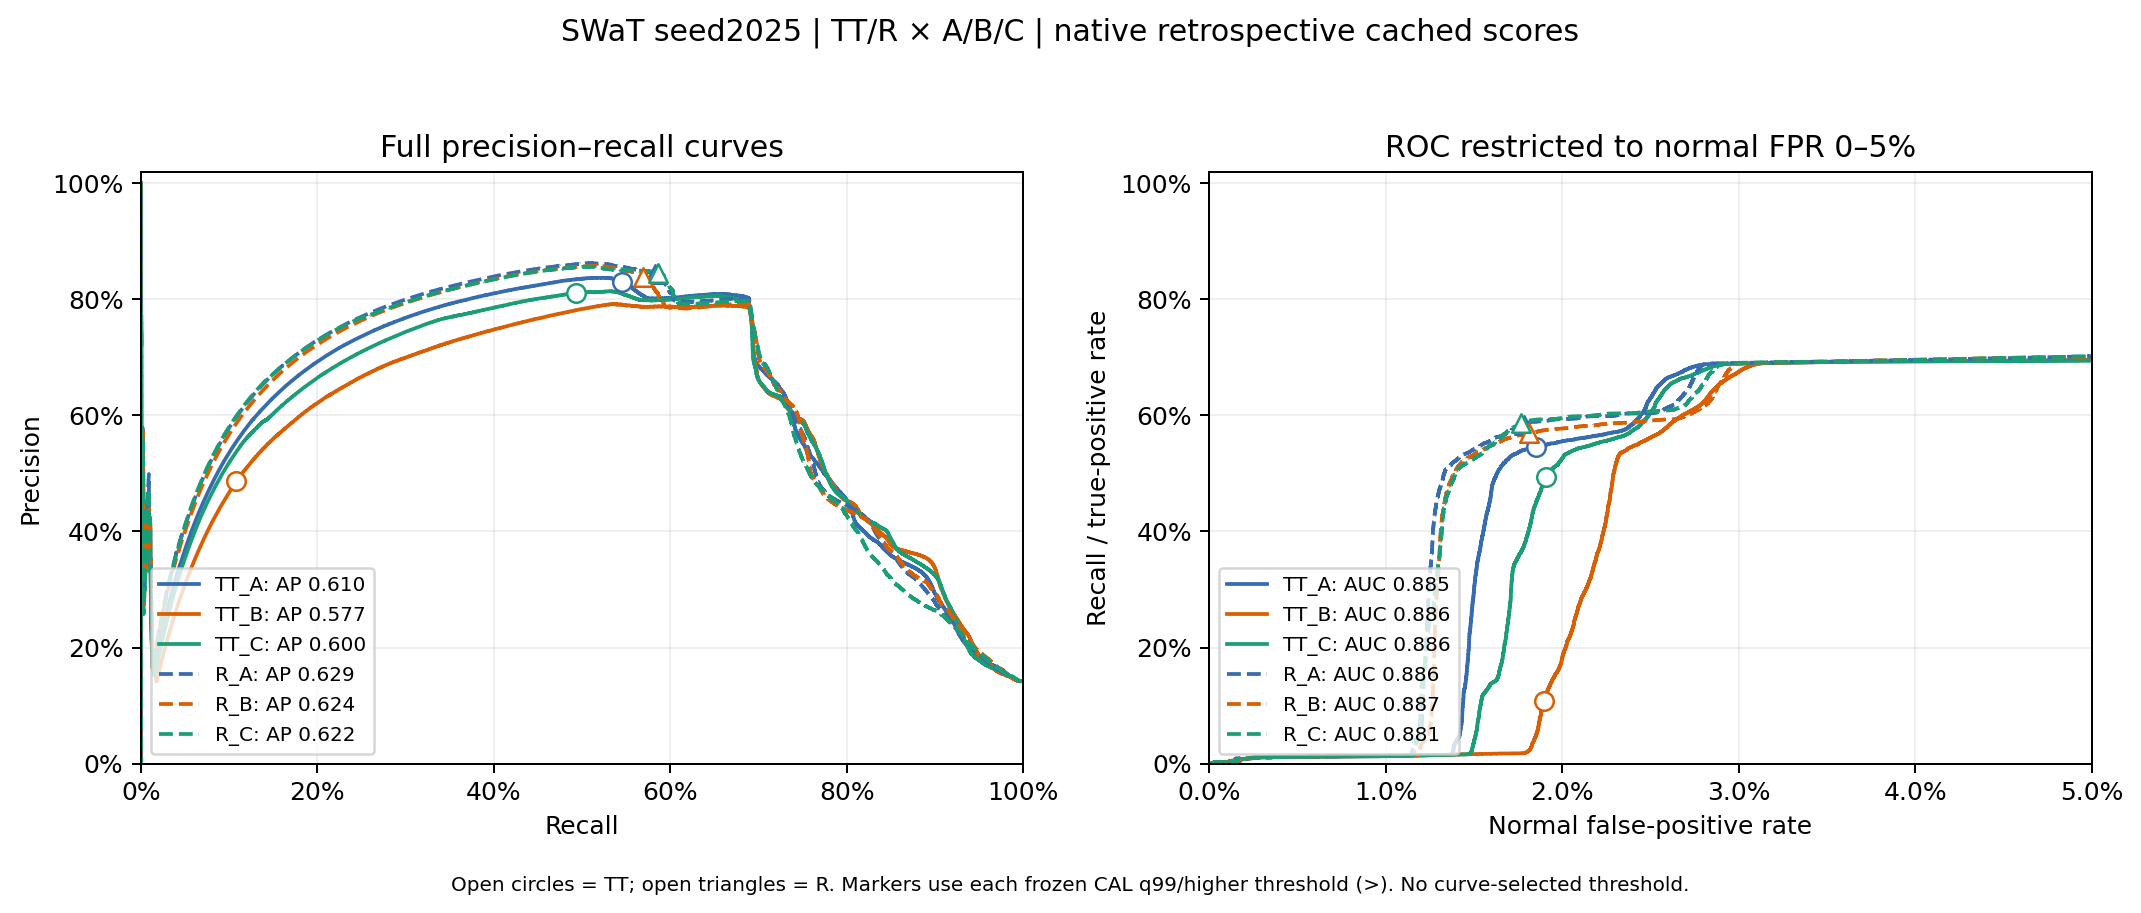
\includegraphics[keepaspectratio,alt={Archived SWaT curves for seed 2025. The original calibration operating points are overlaid on precision-recall and low-FPR ROC curves. The curves describe threshold variation without selecting a new threshold.}]{../../docs/experiments/left_replay_exposure_repeat_20261118/curves/PR_lowFPR_ROC.png}}
\caption{Archived SWaT curves for seed 2025. The original calibration
operating points are overlaid on precision-recall and low-FPR ROC
curves. The curves describe threshold variation without selecting a new
threshold.}
\end{figure}

The seed-2025 SWaT TT-B and TT-C ROC-AUCs are 0.885519 and 0.885894.
Their strict recalls at the fixed rule are 10.829\% and 49.358\%, at
normal FPRs of 1.895\% and 1.906\%. The existing low-FPR curves help
explain why full ROC area alone misses this operating difference. They
cannot identify a unique training or calibration explanation.

\section{Comparison with Existing
Methods}\label{comparison-with-existing-methods}

External comparisons clarify the scope of the paired LEFT findings. The
comparison group includes a plain multilayer perceptron (MLP), CANDI
\citep{candi2026}, and separately archived native TimeRadar head probing
\citep{timeradar2026}. The matching controls change update policies
within a detector. Comparisons between detectors allow additional
differences in model initialization, score definition, update
mechanisms, and available observations. They are reported within each
named protocol rather than merged into a universal leaderboard.

\textbf{Table 6. External comparison permissions.} Within a row, the
corresponding noU and updating arms use that row's fixed protocol.
Published results are not substituted for missing local cells.

\begin{longtable}[]{@{}
  >{\raggedright\arraybackslash}p{(\linewidth - 4\tabcolsep) * \real{0.3333}}
  >{\raggedright\arraybackslash}p{(\linewidth - 4\tabcolsep) * \real{0.3333}}
  >{\raggedright\arraybackslash}p{(\linewidth - 4\tabcolsep) * \real{0.3333}}@{}}
\toprule\noalign{}
\begin{minipage}[b]{\linewidth}\raggedright
Detector
\end{minipage} & \begin{minipage}[b]{\linewidth}\raggedright
Initialization and adaptation permission
\end{minipage} & \begin{minipage}[b]{\linewidth}\raggedright
Readout and comparison scope
\end{minipage} \\
\midrule\noalign{}
\endhead
\bottomrule\noalign{}
\endlastfoot
LEFT & Task-specific normal-source initialization, native source-prefix
scaler including source validation, matched noU/TT/SS/R & 192-point
full-window offline scores, main SWaT/PSM axes \\
Plain MLP & Task-specific source-FIT-only scaler and source-selected
checkpoint, same legal seed-2025 exposure endpoints for its TT/R &
10-point window reconstruction error at its true endpoint, same point
indices as the main comparison \\
CANDI & Same plain MLP source reference, complete selection and residual
module on chronological unlabeled target FIT, frozen at scoring &
10-point endpoint MSE, local fit-then-freeze protocol rather than native
continuous test-time learning \\
TimeRadar & Author-supplied pretrained state including synthetic anomaly
information in pretraining. Project native-variance noU and decoder-only
TT/SS/R & 100-point endpoint variance, distinct PSM 64,728-point query
axis and separate CAL archive. Historical full-window variants have
different time permissions \\
TSAD-C & Published contaminated-training method. Local scorer and
inference compatibility did not qualify & Local results are NA.
Literature only \\
\end{longtable}

The MLP comparison preserves TT/R's corresponding source and target draw
endpoints using the last 10 points of each authorized training window.
It provides a within-backbone check, not a controlled comparison that
isolates the benefit of LEFT's time-frequency representation. In seed
2025, MLP R improves AP over MLP TT by 0.591 pp on SWaT and 14.077 pp on
PSM. On SWaT, MLP R has 96.090\% confirmed normal FPR and 5 one-to-one
matches versus 21 any-hit events. LEFT R has 1.512\% confirmed normal
FPR and 15 matches. On PSM, MLP R has AP 0.631848 and 3.146\% confirmed
complete-event coverage. LEFT R has AP 0.587891 and 61.901\% coverage at
a higher confirmed normal FPR, 9.677\% versus 0.759\%. These quantities
compare the stored operating points and show why an AP improvement under
replay need not imply better coverage. There are no matched MLP B/C
experiments in this study.

CANDI under the local fit-then-freeze schedule does not materially
improve on its own plain MLP reference at the fixed configuration. SWaT
AP changes from 0.783949 to 0.783885 while the confirmed normal FPR
rises from 96.748\% to 97.356\%. PSM AP is 0.604606 for both after
rounding, with unchanged confirmed event coverage. The comparison does
not measure how CANDI would behave when it can update throughout the
query stream as described in its original setting. The full same-axis
seed-2025 table is in Appendix C.

On the separate TimeRadar head-probing protocol, seed-2025 TT loses AP
relative to noU on both tasks. R versus TT adds 5.426 pp on PSM and
loses 0.590 pp on SWaT. PSM AP recovery does not preserve noU's
sustained coverage. This external reference supports keeping the
conclusions specific to the task and detector. It does not supply
additional matched LEFT seeds. The frozen TimeRadar and TimesFM
comparison and its negative direct complementarity result remain
archival references rather than part of the adaptation claim.

\section{Discussion and Limitations}\label{discussion-and-limitations}

\textbf{What the paired comparison identifies.} Replacing the second
target half-batch with source data changes the training distribution
while preserving the update count, batch size, initialization, and the
first target draw. This makes R−TT interpretable as the effect of the
replay policy in a defined experiment. It cannot separate the value of
additional source examples from the effect of giving fewer target
examples the opportunity to influence the detector. R−SS and R−noU help
interpret those comparisons but cannot by themselves prove that replay
prevented internal forgetting. We did not measure a unique parameter- or
representation-level retention mechanism.

\textbf{Task-dependent exposure effects.} A controlled window
replacement isolates changes more tightly than a naturally mixed
before-and-after comparison. The replacement windows still come from a
small number of labeled events and share underlying observations. Their
temporal and multivariate structure can differ from that of nominally
normal replacements. SWaT results show limited protection against this
added exposure. PSM shows a different AP response and lower absolute
event coverage for replay. The interaction is specific to the labeled
donor eligibility, replacement design, exposure level, and remaining
target/source mixture.

\textbf{Operational meaning.} A detector can assign a better global
ranking yet alarm less often on an event in the selected operating
region. Conversely, when its threshold produces nearly continuous
alarms, any-hit and pooled coverage can appear high regardless of useful
event separation. The original q99 rule gives each arm its own threshold
in score units and does not equalize normal false-positive rates. PSM's
all-attack CAL is a particularly severe limit on operating
interpretations. We retain both rank measures and the fixed rule, with
no query-tuned threshold. The offline full-window LEFT readout and
retrospective location and availability metrics cannot establish online
response times.

\textbf{Generalization and comparison limits.} The primary evidence
spans two exposed public development tasks, each with one initialization
and three adaptation seeds. It supplies no independent site, device,
time split, or pretraining replication. Repeated draws and repeated
scoring of the same events do not widen that support. Plain MLP and
CANDI are available at one seed, with unequal window lengths, scalers,
initializers, and learning permissions relative to LEFT. TimeRadar's
separate protocol and the unavailable local TSAD-C result limit breadth.
All files and claims in this study use public datasets. The observed
protection and parameter trade-offs should not be attributed to a
general guarantee against arbitrary contamination, a new anomaly head,
or transferable time-frequency synergy.

\section{Conclusion}\label{conclusion}

On SWaT, ordinary mixed-unlabeled target updating raises ROC-AUC
relative to the frozen detector while lowering AP and calibrated
confirmed coverage. Adding nominally normal source windows to the
adaptation batch improves AP over equal-budget target-only updating in
all six paired comparisons across SWaT and PSM and reduces observed
false-positive points. Replay improves confirmed coverage relative to TT
on SWaT and reduces coverage on PSM. Under the fixed exposure
intervention, the AP protection pattern repeats on SWaT. In PSM,
abnormal replacement raises AP compared with normal replacement in both
arms. These results separate ranking, calibrated alarm cost, event
discovery, and anomaly persistence for an established update policy.

\href{supplement.md}{Supplementary material and linked experiment
records}.

\bibliography{references.bib}

\end{document}
